ergibt%--> Je Subsection Punkt Fragen formulieren.

%-------------------------------------------
% HEADER

% Roterfade der Einleitung:

% 1. Problem -> Kompatibilität
% 2. Ziel -> Lösung mit Übersetzungsprogramm
% 3. Abgrenzung Interpreter & Compiler -> Übersetzungsprogramm als Transpiler
% 4. Formale Grammatike -> Formale Grammatik als Vorrausetzung des Transpilers
% 5. JavaCC -> Implementierung der Formalen Grammtik mit JavaCC und damit des Transpilers

%-------------------------------------------

\section{Theoretische Grundlagen}
\subsection{Problemstellung}
	
Es gibt zwei grundlegende Probleme die eine PL/I zu Java Übersetzung lösen soll. 
Einerseits das Kompatibiltätsproblem von PL/I-Programmen, die auf modernen Platformen laufen sollen, wie etwa Cloud-Instanzen, oder Linux-Server. Andererseits die mit einem hohen Aufwand verbundene Wartung von bestehenden PL/I-Programmen. 
	
Bestehende PL/I Compilerlösungen führen aktuell zu einem Kompatibilitätsproblem. Der PL/I Compiler, der auf den meisten Computer-Systemen im Einsatz ist wird von IBM entwickelt und vermarktet. Hierbei handelt es sich um einen Compiler der expilziet für z/Os geschrieben wurde. Dabei ist z/Os ein Betriebssystem für die von IBM vermarkteten Großrechner. Eine kompilierung von PL/I auf einem herkömmlichen x86-Desktop Computer oder in der Cloud ist mit diesem Compiler nicht möglich. 
(https://www.ibm.com/de-de/products/pli-compiler-family) 

Eine Alternative bietet die Organisation GNU mit der GNU Compier Collection (GCC). Der Entwickler Henrick Sorensen entwickelte Teile des Frontends für einen PL/I Compiler. Dabei verwendete er das Backend, das die GCC zu verfügung stellt. Jedoch gab es bei diesem Projekt seit 2007 keine weiteren Neuerungen mehr. Der Entwickler gibt an, das bisher keine Zwischencode Erzeugung stattfindet, was diesen Compiler bisher unbrauchbar macht. Somit ist dieser Compiler keine Alternative zu dem von IBM.
(https://pl1gcc.sourceforge.net/) 

Heutzutage ist die gängige Möglichkeit, ein IBM 3270 Terminal zu emulieren, das eine Verbindung zu einem z/Os System herstellt, und den PL/I Code auf diesem zu kompilieren.
Weiterhin ist PL/I eine Altsprache, die seit den 1960er Jahren im Einsatz ist und durch den Generationenwechsel an Entwicklern verliert. Wartung und Entwicklung werden so häufig schwer und teuer. (https://dl.acm.org/doi/pdf/10.1145/960118.808389, S.228ff. IBM Watson Research)

Java hingegen ist auf nahezu allen modernen Systemen durch die plattformunabhängige Java Virtual Machine (JVM) kompilierbar. 
(https://docs.oracle.com/cd/E19620-01/805-4031/ch1intro-6/index.html)

Insbesondere ist eine Kompilierung auch auf einem IBM-Großrechner mit z/Os möglich. (https://www.ibm.com/docs/en/zos-basic-skills?topic=zos-java)
Das macht Java zu einer flexibel Einsetzbaren Sprache. Weiterhin is Java die mit am meisten verwendete Programmiersprache in der heutigen Zeit. (https://www.tiobe.com/tiobe-index/) Das führt zu einer höheren Anzahl an Entwickler, die in der Lage sind Java Programme zu warten.

% @review: Begriffswahl
In diesem und den nachfolgenden Kapiteln wird immer wieder zwischen dem Programm unterschieden welches den Quellcode übersetzt, dem Programm welches als Eingabe verwendet wird und das Programm welches als Ausgabe erzeugt wird. Um eindeutig zu differenzieren welches Programm aktuell im Text diskutiert wird, wird das Übersetzungsprogramm als Transpiler bezeichnet, das Eingabeprogramm mit PL/I-Quellcode und das Ausgabeprogramm mit Java-Zielcode umschrieben. 

% Was ist ein Transpiler?
Um nun die Programmiersprache Java für die Lösung der eingangs dargelegten Probleme zu verwenden, wird ein Transpiler benötigt, welcher PL/I-Quellcode in Java-Zielcode übersetzt. Ein solcher Transpiler verarbeitet Quellcode der Sprache PL/I so, dass aus diesem Quellcode der Sprache Java generiert werden kann. Dabei ist es möglich das der Benutzer, selbst wählt wie er welche Ausdrücke übersetzt. Ist der Programmcode erst mal in Java übersetzt worden, kann der Java-Zielcode durch die JVM kompiliert werden.

% Weiterführung
Am Ende ist zwar der PL/I-Quellcode übersetzt und auch kompilierbar, jedoch ist ab diesem Punkt erst die tatsächliche Qualität des Transpilers zu erkennen. Faktoren wie Lesbarkeit und Erweiterbarkeit des Java-Zielcodes gehen in die Beurteilung mit ein. 
Die Beurteilung der Qualität des Transpilers ist auch von Zielaspekten der Benutzer abhängig. In dieser Arbeit wurden Zielgruppen definiert die im nachfolgenden Kapitel 1.2 weiter erläutert werden sollen. Diese Zielgruppen sind für weitere Gestaltungsentscheidungen in der Entwicklung des Transpilers wichtig.

%Anderseits auch die veränderte Laufzeit-Performance. Die Laufzeit-Performance kann durch eine Übersetzung verschlechtert, wie auch verbessert werden. Somit ist nicht nur die reine Übersetzung Teil der Problemstellung, sondern es gilt auch die Übersetzung zu beurteilen. 
\pagebreak
     

% 	 Welches Problem löst das Programm?
%	 Probleme 
%			 1. Nicht auf jedem System läuft PL/I, besonders nicht auf modernen x86 bzw. Cloud.
%			 2. PL/I ist eine weniger verwendete Sprache, Wartung teuer &  Schwer.

%	 (Hinführung zum Problem:
%	 Historisches Kompatibilitätsproblem -> Nicht auf jedem System lief jede Assambler Sprache, Problem: hoher Aufwand und Unflexibel
% 	 Deshalb -> Compiler mit Hochsprache, der Code für das Backend des Compilers, bspw. C's Gcc Compiler
%    in Assambler Sprache des Systems übersetzt.)? **Hier einen Cross Compiler erklären bzw. im Zusammenhang mit dem Historischen Problem.**

%	 Problem mit PL/I -> Pl/I Compiler rar bzw. nur für Großrechner Systeme vorhanden   
%	 Es gibt zwar einen GCC Pl/I Compiler, dieser wird aber seit 2007 nicht mehr weiterentwickelt. Eine Weiterentwiclung könnte auch Interessant %    sein, löst aber nicht das Problem der teuren Wartung von Programmen in PL/I.

% 	 
%	 Lösungsvorschlag zu 1 -> PL/I zu Java Transpiler bauen Java und JVM relativ System unabhängig und damit Ideale Zielsprache für eine 
%	 hohe Kompatibiltätsrate.Um zum Beispiel Pl/I Programm die auf einem Großrechner laufen auch auf einem x86 On-Prem Server oder einer Cloud
%    zu betreiben. **Hier die Frage klären was ein Transpiler ist**
%	 
%    Lösungsvorschlag zu 2 -> Java ist den großteil der Softwareentwickler bekannt und eine Wartung ist leichter.
%
    
\subsection{Zielsetzung}
% Herleitung von der Problemstellung	
Das Ziel dieser Arbeit leitet sich aus der eingeführten Problemstellung in Kapitel 1.1 ab. Allgemein soll ein plattformunabhängiger Transpiler entstehen, der die  Entwicklung und Transformation von PL/I-Quellcode ermöglicht. Die zugrundeliegende Arbeit stellt die Entwicklung, sowie die Gestaltung der Software dar und wird schlussendlich diskutiert. 

% @review: Referenz zur Begriffklärung
% Zielgruppen Zusammengefasst	
Somit richtet sich diese Arbeit und der Transpiler teils an für juniore Anwendungsentwickler in den Sprachen PL/I bzw. Java. Für diese Nutzergruppe soll der Transpiler ein Hilfswerkzeug darstellen. Nachfolgend werden diese als Benutzer bezeichnet. Eine andere Nutzergruppe sind Administratoren, die den Transpiler selbst anpassen und erweitern möchten. Ermöglicht wird dies durch eine modulare Architektur. Auch bei den Zielgruppen, werden in den nachfolgenden Kapiteln explizit die definierten Begriffe verwendet um den etwaigen Zweck einer Entwicklungsentscheidung zu diskutieren.
	
% Junior Entwickler die gerade in PL/1 einsteigen.
Juniore Entwickler profitieren von dieser Arbeit als Einstiegspunkt in die Programmiersprache PL/I. Dadurch das es schwierig ist PL/I-Quellcode auf einem herkömmlichen Desktop Computer zu kompilieren, soll der erarbeite Transpiler Abhilfe schaffen. Beispielhaft könnten Entwickler den Transpiler als Test-Umgebung für den eigenen entwickelten PL/I-Quellcode verwenden.

% Lernhilfe
Für Benutzer, die mehr Erfahrung mit Java haben, eignet sich der Transpiler als Lernhilfe. Es wird ihnen so erleichtert, PL/I-Quellcode zu analysieren. Sie können bestehende Kenntnisse aus Java anwenden, um gleiche Muster in PL/I wiederzuerkennen. Dies kann den Lernprozess beschleunigen. In dieser Arbeit wird dabei die Gestaltung von Übersetzungsmustern, des zugrundeliegenden Transpilers diskutiert. Hierzu wird an Vor- und Nachteile gewählter Gestaltungen herangeführt.

% Benutzbarkeit
Der Transpiler aus der Projektarbeit-IV konnte bisher über die Kommandozeile, sowie der IDE Eclipse verwendet werden. Diese ursprüngliche Benutzung des Transpilers führte zu einer erhöhten Fehleranfälligkeit und Dokumentationsbedarf. Ein vereinfachtes Darstellungskonzept, welches in Kapitel 2.? Vorgestellt wird, bietet  Benutzern einen leichteren Einstieg in das Programm.
Die Komplexität der Benutzung wird durch ein Graphical-User-Inferface (GUI) vereinfacht. Das Konzept dieser GUI soll dem eines Übersetzers der natürlichen Sprache, wie etwa 'DeepL' oder 'Google-Translate', ähneln. Mit diesen Konzepten sind Benutzer vertraut, erleichtert den Einstieg in die Programmiersprache PL/I, das Testen des PL/I-Quellcode, sowie die schnelle Übersetzung.

%  Entwickler die das Programm eigenständig erweitern, verändern wollen.
Durch die modularisierte Gestaltung des Transpilers können Administratoren selbst Module austauschen und erweitern, etwa durch eine API-Schnittstelle zu externen Übersetzungsbibliotheken/-services. 

%  Zusammenfassung und hinführung zum nächsten zu dem Unterschied Interpreter und Compiler
Auch wenn beide Zielgruppen unterschiedliche Ausprägung der Zielvorstellung haben, wollen beide eine Übersetzung von einer Quellsprache in eine Zielsprache erreichen. Die Gestaltung eines Übersetzers erfolgt dabei unabhängig davon ob es sich um PL/-Quellcode und um Java-Zielcode handelt. Ein Übersetzer kann sowohl als Interpreter und als Compiler gestaltet werden. In dem nachfolgenden Kapitel 1.3 werden die Begriffe voneinander abgegrenzt. 
	
% Aufteilung der Zielstellung:
% 1. Allgemein; Ableitung aus der Problemstellung
% 2. Zielgruppen spezfifisch
% 2.1 Einfache und unkomplizierte Lösung
%
% 2.2 Erweiterung des Transpilers bzw. ersetzen von Modulen	
	
% - Wie eine Art JavaScript Minifier oder 
%  Wer ist die Zielgruppe?
%  - Junior Entwickler die gerade in PL/1 einsteigen.
%   - Lernhilfe
%  - Online-Smoketest von PL/I Code
%   - Benutzbarkeit
%   - Entwickler die das Programm eigenständig erweitern, verändern wollen.
 
%  Ziele der Architektur (Zielgruppe Entwickler)
%  - Perspektive des Entwicklers
%  - Perspektive des Benutzers
    \pagebreak

\subsection{Abgrenzung Interpreter und Compiler}
% Wie können Programme ausgeführt werden?
Für die nachfolgenden Kapitel soll in diesem Kapitel ein Transpiler bzw. Source-to-source Compiler von einem Interpreter abgegrent werden. Um die Unterschiede deutlich zu machen sollen die Formen von Übersetzungsprogrammen, wie die des Compilers und Interpreters voneinander abgerenzt werden. 
  
% Wie arbeitet ein Compiler?
Ein Compiler besteht aus einem Frontend und einem Backend. Das Frontend umfasst die lexikalische Analyse, die syntaktische Analyse, die semantische Analyse und die Symboltabelle, die in jedem dieser Schritte verwendet wird. 
Das Ergebnis des Frontends ist eine Zwischencodedarstellung. Diese Zwischencodedarstellung wird an das Backend übergeben, um daraus Maschinencode zu generieren. Der Maschinencode kann dann auf dem zugrundeliegenden System ausgeführt werden. (Compilers: Prinicples and Techniques, S. 106ff.)
Um weiterhin den Prozess der übersetzung mithilfe eines Compilers darzustellen, wird Abbildung ?.? verwendet.

\pagebreak
% @todo: Hier evtl. Abbildung...
\begin{figure}[h]
  \centering
  \caption{Funktionsweise eines Compilers}
  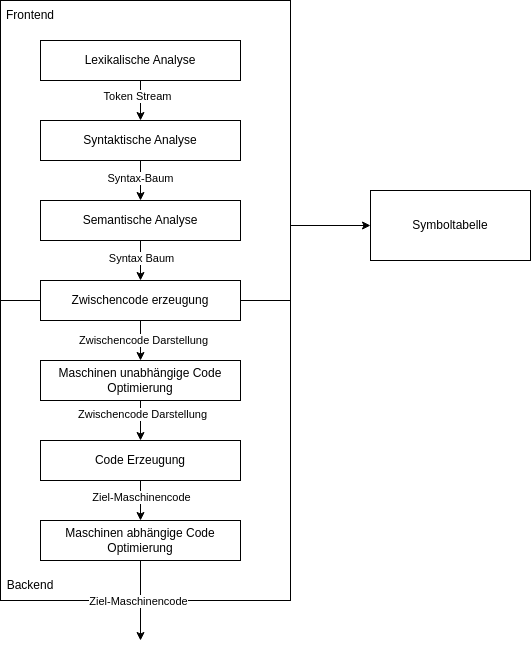
\includegraphics[scale=0.75]{compiler-ablauf-diagramm.png}
  \label{fig:compiler}
\end{figure}
\pagebreak
Abbildung ?.? zeigt eine Übersicht und das Ergebnis der einzelnen Phasen. Die Abbildung unterteilt den Ablauf wie eingangs beschrieben in Frontend und Backend.

In der ersten Phase teilt der Compiler den eingegebenen String in Tokens auf. Danach entsteht ein Syntaxbaum, der in eine Zwischencodedarstellung umgewandelt wird. Ab diesem Punkt beginnt das Backend des Compilers. Zuerst erzeugt es maschinenunabhängigen Code und anschließend maschinenabhängigen Code. Dieser maschinenabhängige Code ist auf dem zugrundeliegenden System ausführbar. (Compilers: Principles and Techniques, s. 30) 

%  Warum ein Transpiler?
Ein Compiler kann in unterschiedliche Art und Weise implementiert werden, wobei die Ausprägung der Prozessschritte, wie beispielsweise das Ergebnis der syntaktischen Analyse, häufig variiert. Es ergeben sich folglich Methoden den Compiler zu konstruieren.

Ein One-Pass-Compiler erzeugt keinen Zwischencode, sondern führt den Code direkt aus. Diese Methode wurde ursprünglich angewendet, um Speicherplatz zu sparen, da frühe Computer nur begrenzte Kapazitäten hatten und keine Zwischenergebnisse speichern konnten. Ein Beispiel für eine Sprache, die mit einem One-Pass-Compiler kompiliert wird, ist Turbo Pascal. (https://keleshev.com/one-pass-compiler-primer)

Diese Bauweise eines Compilers eignet sich nicht für den zu entwickelten Transpiler. Da es nicht das Ziel des Programms ist, den PL/I-Quellcode schnellstmöglich auf einem System in Binärcode umzuwandeln und auszuführen. Stattdessen liegt die Übersetzung im Vordergrund.

Eine weitere Methode einen Compilter zu entwickeln, ist ein Source-to-Source Compiler.
Dieser unterscheidet sich durch die Zielsprachen, in die er übersetzt. Während ein C-Compiler den C-Code nach der Zwischencodeerzeugung in Assemblersprache und anschließend der Assembler den C-Quellcode in Maschinencode übersetzt, wandelt ein Source-to-Source-Compiler beispielsweise C-Quellcode in Java-Zielcode um. 
Diese Vorgehensweise ist deckungsgleich mit der des entwickelten Transpilers. Lediglich das von der Hochsprache PL/I in die Hochsprache Java übersetzt wird.

Abbilding ?.? zeigt die Prozessschritte eine Transpilers.

\pagebreak
\begin{figure}[h]
  \centering
  \caption{Funktionsweise eines Transpilers}
  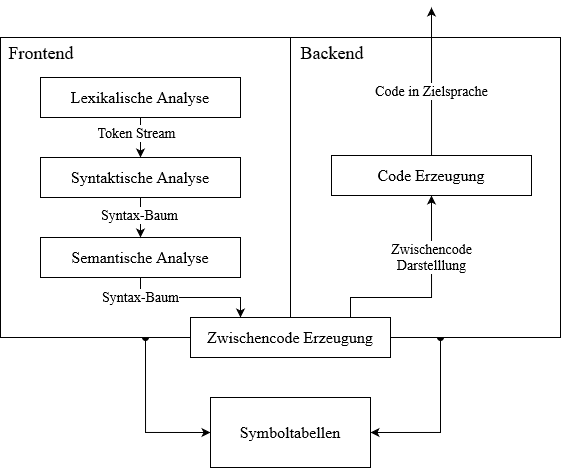
\includegraphics[scale=0.75]{transpiler-diagramm.png}
  \label{fig:transpiler}
\end{figure}
\pagebreak

Ein Vergleich von Abbildung ?.? mit Abbildung ?.? zeigt, dass die ersten Phasen bis zur Zwischencodeerzeugung gleich bleiben. In Abbildung ?.? sind jedoch die Prozesse des Frontends neben denen des Backends dargestellt. Diese Darstellung soll die unterschiede der Sprachebenen bei einem Transpiler und einem Compiler verdeutlichen.

Wie schon beschreiben übersetzt ein Compiler den Quellcode einer Hochsprache in eine maschinennahe Sprache wie Assembler. Ein Transpiler hingegen behält die Sprachebene der Quellsprache auch bei der Zielsprache bei. In Abbildung ?.? werden zudem die Phasen des Backends reduziert, da keine Übersetzung in eine maschinenabhängige Sprache erforderlich ist.

% @review
Deutlich wird auch der Unterschied zwischen Compiler und Transpiler, durch das Ergebnis der jeweiligen Übersetzung. 
Das Ergebnis der Übersetzung eines Compilers ist Binärcode der auf einem Zielsystem ausgeführt werden kann. Um hingegen das Ergebnis eines Transpilers auszuführen,
braucht es einen weiteren Compiler. Dieser Compiler muss den Zielcode der Zielsprache in Binärcode übersetzen und ausführen können.
Bei der übersetzung von PL/I-Quellcode zu Java-Zielcode, bedarf es also einen weiteren Java-Compiler der den Java-Zielcode in Binärcode übersetzt 
und damit ausführbar macht.  

% @review: Cross Compiler? - Hat hier eig nix zu suchen, ist Thema für Boostrapping aber nicht für Transpiler
Neben den Methoden der Konstruktion, gibt es auch unterschiedliche Verwendungen. 
Etwa existiert der Begriff der Cross-Kompilierung. Hierbei handelt es sich um die Möglichkeit einen Compiler, der sich auf einem externen Computersystem befindet zu verwenden um den Quellcode auf dem lokalen System in Binärcode zu übersetzen. (https://www.gnu.org/software/automake/manual/html_node/Cross_002dCompilation.html) 
Diese Verwendungsweise findet etwa Anwendung beim Bootstrapping. Liegt auf dem System noch kein Compiler für die Sprache vor, in der der Kernel geschrieben wurde, wird diese Methode verwendet um den Kernel-Code zu kompilieren. 
In dieser Arbeit kommt ein solcher Ansatz bedingt zum Einsatz. Wird der Transpiler in einem Webinterface verwendet, ist die Verhaltensweise ähnlich.
Da auch hier der Compiler auf einem anderen Host-Computer, den lokalen Quellcode übersetzt. Jedoch nicht in Binärcode. 
Der Transpiler lässt sich jedoch problemlos auch auf einem lokalen System verwenden. Bei einem Cross-Compiler, ist die komplitibiltät mit dem lokalen System von der Rechner-Architektur abhängig.

Sowohl One-Pass-Compiler, Transpiler bzw. Source-to-source Compiler als auch herkömmliche Compiler übersetzen das Programm basierend auf seiner Gesamtstruktur. (https://keleshev.com/compiling-to-assembly-from-scratch/excerpt-compiling-to-assembly-from-scratch.pdf)[S. 18ff.] 
Eine Alternative ist der Interpreter. Dieser führt den Quellcode direkt Zeile für Zeile aus.

% Wie arbeitet ein Interpreter?
Im Vergleich zu einem Compiler hat der Interpreter weder ein Frontend noch ein Backend. Es gibt keine klare Trennung zwischen einem Frontend, das eine unabhängige Repräsentation des Codes erzeugt, und einem Backend, das diese Repräsentation interpretiert. 

Programmiersprachen, die von einem Interpreter ausgeführt werden, sind beispielsweise PHP3, Ruby und JavaScript. Weiterhin wird ein Interpreter auch durch die Shell verwendet um Benutzerbefehle zu verarbeiten. Es ist auch möglich, sowohl einen Interpreter als auch einen Compiler für die Übersetzung bzw. Ausführung von Quellcode zu verwenden. Die Sprache 'Go' beispielsweise nutzt sowohl einen Compiler als auch einen Interpreter. Dabei wird das Go-Programm mit dem Befehl \verb+go build+ kompiliert und mit \verb+go run+ sofort durch den Interpreter ausgeführt. (https://craftinginterpreters.com/a-map-of-the-territory.html)
Um die Funktionsweise eines Interpreters besser mit der des Compiler zu vergleichen, soll die Verwendung eines Interpreters durch die Shell näher betrachtet werden. Eine Shell wird auf unixoiden und MS-DOS Betriebssystemen eingesetzt.
  
% Absatz: Ein Interpreter am Beispiel von Bash
Auf unixoiden Betriebssystemen dient die Shell als Interpreter für Skriptprogramme. Sie nimmt Benutzerbefehle direkt oder aus Skriptdateien entgegen und übergibt sie zur Ausführung an das Betriebssystem. Außerdem übernimmt sie die Ausgabesteuerung und kontrolliert die Datenströme. 
Um Befehle zu verarbeiten werden Interpreter Lösungen verwendet wie, \verb+bash+, \verb+csh+, \verb+zsh+ oder \verb+Powershell+.

% @review: Was unterscheidet die Shell von einem Übersetzer(Compiler)
Shell ist keine Programmier- oder Skriptsprache. Hingegen bringen die genannten Interpreter, Erweiterungen mit, die einer Programmiersprache ähneln. Bei \verb+bash+ werden etwa Programmiersprachen-ähnliche Konstrukte, wie Variablen, Kontrollstrukturen oder Funktionen verwendet. (https://www.gnu.org/software/bash/manual/bash.html#What-is-a-shell_003f)

In der Linux Manual Page wird \verb+bash+ auch als Command-language Interpreter bezeichnet. (https://www.man7.org/linux/man-pages/man1/bash.1.html)
Jedoch ist der allgemeine Zweck einer Shell immernoch die Verarbeitung von Befehlen und das ausführen von kompilierten Programmen.
Um den Unterschied zwischen einem Interpreter, wie bash, und einem Compiler zu verdeutlichen, wird in Abbildung ?.? die Arbeitsweise des Interpreters von bash dargestellt.

Abbildung 1.1 stellt den Ablauf der Skript-Interpretation dar.
\begin{figure}[h]
  \centering
  \caption{Ablauf der Interpretation eines Shell Programms}
  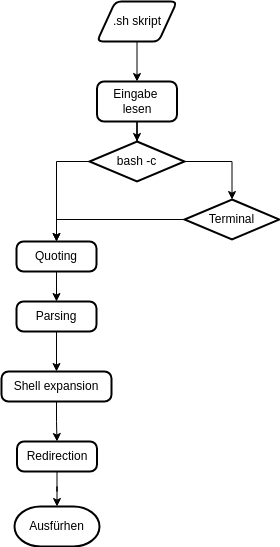
\includegraphics[scale=0.75]{shell_interpreter.png}
  \label{fig:shell}
\end{figure}
\pagebreak

Die Eingabe des Bash-Skripts wird zeilenweise gelesen, entweder über ein Terminal oder durch den Befehl \verb+bash -c+. Beide Eingabemethoden führen zur ersten Phase von Bash.

Die Phase das Quoting folgt dem Prinzip der lexikalischen Analyse, bei der alle Sonderzeichen entfernt werden, wie zum Beispiel Kommentare oder Backslashes. Sobald das Quoting abgeschlossen ist, entsteht ein String, der nur aus den Tokens eines Ausdrucks besteht.

Anschließend beginnt das Parsing, das der syntaktischen Analyse im Kompilierprozess ähnelt, jedoch keine Zwischencodeerzeugung beinhaltet. Hier wird lediglich zwischen einfachen Befehlen und zusammengesetzten Befehlen unterschieden. Einfache Befehle umfassen das Ausführen der integrierten Shell-Programme wie \verb+ls+, \verb+wc+ oder \verb+mkdir+. Zusammengesetzte Befehle bringen zusätzliche Logik in das Bash-Skript ein, wie zum Beispiel \verb+if+, \verb+while+ oder \verb+case+.

Der Verarbeitungsprozess setzt sich mit der Shell-Expansion fort, bei der in einem Befehl eingebettete relative Ausdrücke durch ihre absoluten Repräsentationen ersetzt werden. Zum Beispiel würde im Ausdruck \verb+echo ${pwd}+ das \verb+$pwd+ durch den absoluten Pfad des aktuellen Verzeichnisses ersetzt.

Schließlich wird der des ausgeführten Skripts durch die \verb+stdio+-Bibliothek ausgegeben, in der Kommandozeile ausgegeben.
(https://www.gnu.org/software/bash/manual/bash.html#Shell-Operation)

% Absatz: Zusammenfassende Unterscheidung zwischen Interpreter und Transpiler, Was sind gemeinsamkeiten und unterschiede von Transpiler und interpreter?

Zusammenfassend zeigen sich sowohl Ähnlichkeiten als auch Unterschiede zwischen einem Interpreter und einem Compiler. Beide durchlaufen die Phasen der lexikalischen und syntaktischen Analyse, wobei sie den Quellcode zunächst bereinigen, um Kommentare, Leerstellen oder andere für die Übersetzung irrelevante Symbole. Anschließend erfolgt entweder die direkte Übersetzung des Quellcodes oder die Erzeugung einer unabhängigen Repräsentation.

% Der entscheidende Unterschied liegt darin, dass der Interpreter den Quellcode lediglich zeilenweise direkt übersetzt, während der Compiler das Programm in eine andere Form transformiert und liest. Dabei stehen die verwendeten Ausdrücke des Eingabecodes in Beziehung zueinander, beispielsweise durch die Verschachtelung von Verzweigungen und Schleifen.

In diesem gesamten Prozess werden ausschließlich Bash-Befehle verwendet. Der Quellcode wird nicht von einer Hochsprache in eine Assamblersprache oder eine andere Hochsprache umgewandelt. Dies verdeutlicht einen zentralen Unterschied zwischen einem Interpreter und einem Compiler: Es entsteht keine Repräsentation des Codes in einer anderen Sprache. Vom lesen des Quellcodes bis zum ausführen des Programms bleibt der Interpreter bei einer Sprache. 

Um PL/I-Code korrekt in Java zu übersetzen, sind Verbindungen zwischen den Ausdrücken wichtig. Eine bloße zeilenweise Übersetzung könnte zu einem Java-Programm führen, das kaum objektorientierte Paradigmen enthält. Der Transpiler sollte eine solche Repräsentation darstellen können.
Allgemein sei zu erwähnen das es möglich ist einen Interpreter für die Übersetzung zu verwenden, dies ist jedoch nicht Bestandteil dieser Arbeit.

Wie schon in den Abbildungen ?.? und ?.? dargestellt sind die ersten Arbeitsschritte des Transpilers die lexiklaische und syntaktische Analyse.
Für beide Prozesschritte werden ein Parser und Lexer benötigt. Mit einem Compiler-Compiler können diese Module mit einer formalen Grammatik generiert werden.
Das folgende Kapitel beleuchtet Grammatiken formaler Sprachen wie PL/I und Java genauer.

% - Erweiterung des Umfangs während der Laufzeit
% - Trennung Laufzeit/Konzeptionsphase

% - Hier erwähnen das eine geminsamkeit die definition von Grammatiken ist, dann überleiten zu Formale Grammatiken.
% - Auch Entscheidung treffen was genau der Transpiler ist, Compiler oder Interpreter
\pagebreak
   
   
\subsection{Formale Sprachen und ihre Grammatiken}
% Warum braucht ein Compiler eine Grammatik?
In dem vorangegangen Kapitel wurden unterschiedliche Methoden, Anwendungsgebiete und Formen der Sprachinterpretation eines Computers vorgestellt. Damit die Interpretation von Sprachen korrekt erfolgt, braucht ein Computer Regeln. Grammatiken beinhalten diese Regeln. Damit der Transpiler korrekt arbeitet wird eine definierte Grammatik benötigt. Nur so können die Prozessschritte der Lexikalischen- und der Syntatkischen Analyse korrekt erfolgen. Denn diese Schritte prüfen den eingegeben Quellcode auf seine grammartikalische Richtigkeit. Bevor also die Sprachliche Analyse erfolgen kann, sollte eine Grammatik angwendet werden.
	
% Woraus besteht eine Grammatik?
Um eine Grammatik anzuwenden muss klar sein, um welche Grammatik es sich handelt. Weiterhin sollte bestimmt werden welche Art von Sprache beschrieben werden soll. 
Eine formale Sprache unterscheidet sich von einer natürlichen Sprache in der Anwendungsform. Die Anwendung von solchen Sprachen dient der logisch präzisen Beschreibung von Ausdrücken. (introduction to formal languages and automata, S. 149ff.) Eine Grammatik besteht aus Variablen, Terminalsymbolen, einen Startsymbol und einer Produktion. Zusammengefasst in:

\begin{center}
\begin{equation}
G=(V,T,S,P)
\end{equation}
\end{center}

Hierbei \verb+V+ für Variablen bzw. Nicht-Terminalsymbole, \verb+T+ für Terminale, \verb+S+ für Start und \verb+P+ für Produktion steht. Dabei ist \verb+S+ ein Teil von \verb+V+. (introduction to formal languages and automata, S. 31ff.)


% @review: Keine Hierachie Einordnung, ledilgich nennen das es sie gibt.
% Welche Typen von Grammatiken gibt es? Chomsky Hierarchie
Grammatiken lassen sich weiter durch die Chomsky Hierarchie spezifizieren. Noam Chomsky unterteilt Grammatiken in vier Ebenen. Ebene null beschreibt unbeschränkte-, Ebene eins kontextsensitve-, Ebene zwei kontextfreie- und Ebene drei reguläre Grammatiken.(https://hpi.de/friedrich/teaching/units/grammatiken.html) 

\pagebreak

Um eine Grammatik darzustellen werden Ableitungen von Produktionen verwendet. In Listing ?.? ist die Produktion einer einfachen \verb+if+ und \verb+else+ Verzweigung dargestellt.

% @todo: PL/I Verwenden und Kontext herstellen
\begin{center}
\begin{equation}
S \to \mathbf{if}\: expr\: \mathbf{then}\: stmt\: \mathbf{else}\: stmt\: | \mathbf{if}\: expr\: \mathbf{then}\: stmt;
\end{equation}
\begin{equation}
expr \to expr\: op\: term\: | term
\end{equation}
\begin{equation}
op \to \mathbf{>}\: |\: \mathbf{<}\: |\: \mathbf{=}\: |\: \mathbf{!}
\end{equation}
\begin{equation}
term \to term\: multOp\: factor\:
\end{equation}
\begin{equation}
factor \to \mathbf{id}\: |\: \mathbf{constant} 
\end{equation}
\end{center}
 
Mit der beschriebenen Grammatik ist folgender Ausdruck zulässig.

\begin{verbatim}
IF A > B THEN 
	CALL proc_1;
ELSE 
	CALL proc_2;
END
\end{verbatim}

Nicht zulässig ist hingegen.

\begin{verbatim} 
CALL IF THEN A > B proc_1;
\end{verbatim}

% @todo: Beispiel-Parsebaum analyse, https://en.wikipedia.org/wiki/LR_parser 
	
% Wie werden Grammtiken in einem Transpiler Programm verwendet?
Die bisher definierten Grammatiken sind in dem Sinne von Bedeutung, weil die Lexikalische und Syntaktische Analyse des Transpilers aus einer solchen Grammatik erzeugt werden. Mithilfe eines Compiler-Compilers kann aus einer repräsentation einer formalen Grammatik ein Parser definiert werden.
 
Für den PL/I-Transpiler bedeutet, dass die aktuelle PL/I-Grammatik für den Parser definiert werden muss. Die aktuellste Grammatik wird durch IBM, in der PL/I Language Referenz definiert. Aus dieser wird mithilfe von JavaCC ein Parser erzeugt. Weshalb in dem folgenden Kapitel 1.5 der Compiler-Compiler und die dazugehörige Grammatik näher beschrieben wird.

% - Theoretischer Abriss
% - Einordnung der resultate der PA 4
%- PL/1 Syntax Wo zu finden? Welche Version der Sprache? 
%	- Reguläre Ausdrücke Syntax, Beispiel einer Grammatik die ich mit verwende, Typ einer Grammatik
%  - Literatur
%    - Chomsky Hierarchie Bücher
%    - https://www-igm.univ-mlv.fr/~berstel/LivreCodes/Codes.html
%  - Woraus besteht eine Grammatik?
%   - Wie lassen sich Grammatiken der Komplexität nach anordnen?
%  - Chomsky Hierarchie
%  Erst Chomsky Hierachier, dann nach Komplexität einordnen und am Beispiel von Regulären Ausdrücken und PL/I Grammatik einführen.
     
\subsection{Anwendung von Formalen Grammatiken in JavaCC}
% 1. Was ist ein Compiler-Compiler? (Verbindung von formalen Grammatiken zu JavaCC)

Nachdem in formale Grammatiken eingeführt wurde, soll nun näher beschrieben werden welche Rolle diese in der Entwicklung des Transpilers spielen.

Der Lexer der die lexikalische Analyse und der Parser, der die Syntaktische Analyse durchführt werden durch JavaCC erzeugt. 
JavaCC ist ein Compiler-Compiler der aus einer formalen Grammatik einen Lexer und einen Parser generiert. 
In Kapitel 1.3 wurde bereits in die Thematik der formalen Grammatiken eingeführt, in diesem Kapitel wird nun die praktische implementation dieser Grammatiken im Zusammenhang mit dem Transpiler beschrieben.

Ein Compiler-Compiler ist eine Technologie mit der aus einer formalen Beschreibung einer Grammatik ein Lexer und ein Parser erzeugt werden. 
Der Lexer und der Parser wenden die in der Grammatik definierten Regeln an und verarbeiten entsprechend die übergebenen Ausdrücke.
Die Darstellung der Grammatik erfolgt in der Regeln in einer Art erweiterten Backus-Naur-Form (EBNF). 
Beispielhafte Compiler-Compiler sind neben JavaCC, Yacc, Antlr und Lexer.
In Kapitel 1.3 wurde bereits vereinfacht eine Produktion aus der PL/I-Grammatik dargestellt. Ähnlich erfolgt auch die Darstellung in einer Grammatikdatei. Folgendes Beispiel zeigt die Darstellung eines \verb+IF ELSE+ Ausdrucks. 
(https://javacc.github.io/javacc/)

\begin{verbatim}
void if_statement() #IF :
{}
{
  < IF > bool_expression() (bool_operation() bool_expression() )*
  < THEN >proc_body()
  [< ELSE >
  	proc_body()]
  	
}
\end{verbatim}

In JavaCC besteht die Möglichkeit die Beschreibung von Produktionen in Methoden zu Kapseln.
In Zeile 1 ist der Methodenkopf zu sehen. In diesem Fall erzeugt die Methode \verb+if_statement+ keinen Rückgabwert.
Das durch die Raute gekennzeichnete Symbol ist die Repräsentation im Parsebaum und zusätzlich auch die Darstellung im Zwischencode.
Im Körper der Methode wird der If-Ausdruck weiter definiert. Terminalsymbole werden in der JavaCC Grammatik mit den größer-als und kleiner-als Zeichne umrandet. Die Nicht-Terminalsymbole hingegen sind wie im Listing ?.? dargestellt weitere Methoden, die wiederum weitere Ausdrücke beschreiben.
Ähnlich wie bei der Produktion aus Listing ?.?, so lange bis lediglich Terminalsymbole übrig bleiben.
Die Methode \verb+bool_expression+ etwa, beschreibt einen zulässigen Boolschen Ausdruck, der durch einen weiteren boolschen Operator mit einem weiteren booleschen Ausdruck verknüft werden kann.
Letzter Ausdruck, kann Leer sein und beliebig oft wiederholt werden. Das ermöglicht komplexe boolsche Operationen.

Weiterhin wird in der Methode \verb+proc_body+ beschrieben welche Ausdrücke in dem Verzweigungskörper zulässig sind. Dazu zählt bspw. auch eine weitere \verb+IF ELSE+ Verzweigung. So werden auch verschachtelte Ausdrücke möglich.
Werden nach und nach die Methoden durch den Compiler-Compiler aufgerufen, ergibt sich eine Regel für Verzweiguns-Ausdrücke. Nach diesem Prinzip ist die gesamte Grammatik gestaltet. 
Die Wurzel aller Methoden, die einen Ausdruck beschreiben, ist dabei die Wurzel Methode \verb+program+, welche das gesamte Programm darstellt. Eine solche Kapselung macht die Grammatik übersichtlich.
Aus dem definierten Ausdruck aus Listing ?? wird schlussendlich ein Parsebaum erzeugt, der durch die Module des Transpilers weiter verarbeitet wird.

% Warum ein Compiler-Compiler verwenden?

Ein Compiler-Compiler generiert somit einen fertigen Parser, aus einer Datei in der eine Grammatik beschrieben wird. Nun gibt es auch die Möglichkeit einen Parser und Lexer selbst zu programmieren. In der Version aus der Projektarbeit-4 wurde ursprünglich ein selbstgeschriebener Lexer verwendet.
Jedoch birgt dieses Vorgehen einen Nachteil. Die Grammatik für den Transpiler ist an zwei stellen definiert und muss somit auch an zwei Stellen gewartet werden.
Wird in die Grammatikdatei für den Parser ein neuer Ausdruck hinzugefügt, muss dieser Ausdruck auch durch den Lexer verarbeitet werden können.
Ursprünglich musste so der Lexer angepasst werden und die Grammatikdatei für den Parser. 
Das führte zu einem erhöhten Arbeitsaufwand und Fehleranfälligkeit. Schlussendlich wurde der selbstgeschriebene Lexer entfernt und der von JavaCC definierte Lexer verwendet.
Somit ist ein Compiler-Compiler gut dazu geeignet den Arbeitsaufwand für die Entwicklung eines Compilers, bzw. eines Transpilers zu reduzieren. 
Es lohnt sich auch bei der Entwicklung auf bereits definierte Resourcen zurückzugreifen. 
Grammatiken für Cobol und Java wurden bereits von der JavaCC Community bereitgestellt. (https://javacc.github.io/javacc/)
Im Fall von PL/I ist keine Grammatik vorhanden. Weshalb bei der Entwicklung des Transpilers, die IBM Language Reference für PL/I die Hauptquelle für die Grammatikdatei ist.   

% @todo: Beschreibung hinzufügen
\begin{tabular}[h]{l|c|r}
Klasse & Beschreibung \\
\hline
JJTPl1ParserState.java & ... \\
Node.java & ... \\
ParseException.java & ... \\
Pl1Parser.java & ... \\
Pl1ParserConstant.java & ... \\
Pl1ParserTokenManager.java & ... \\
Pl1ParserTreeConstants.java & ... \\
SimpleCharStream.java & ... \\
SimpleNode.java & ... \\
Token.java & ... \\
TokenMgrError.java & ... \\
parser.jjt & ... \\
\end{tabular}


JavaCC generiert dynamisch den eigentlichen Parser, hier Pl1Parser, den TokenManager und die ParserConstants Klasse. Die restlichen Klassen sind Boilerplate-Code und werden bei jeder Grammatik generiert. Diese werden auch nur beim initalen kompilieren generiert. Eine weitere Erläuterung des Prasers für den Transpiler ist in Kapitel ?.?

% Wie wird JavaCC in die Entwicklung des Transpiler eingebunden ? (Hinleitung zur Architektur beschreibung)
Durch die Verwendung des JavaCC Jjtree-Moduls, kann global innerhalb des Projekts auf den Parse-Baum zugegriffen werden. 
Der Prase-Baum wird unteranderem durch die Module verwendet, die die Semantische-Analyse und -Synthese repräsentieren.
Erst durch diese wird der Java-Code erzeugt.
Ebenfalls wird für den Parser ein File-Stream benötigt, ein Scanner liefert solchen.
Neben den Parser werden also weitere Module verwendet um schlussendlich den Java-Code für den Benutzer bereitzustellen.
Die gesamte Architektur des Transpilers und dessen weitere Module wird in dem nachfolgenden Kapitel betrachtet. 
Hier werden auch die Technologien vorgestellt die neben JavaCC verwendet werden. 

\section{Technisches Vorgehen}
\subsection{Techstack}
%- Compiler Compiler -> JavaCC: Präsentation, Integration in das Projetk, Grund für die Wahl der Technologie
In Kapitel 1.4 wurde bereits mit JavaCC eine Technologie vorgestellt. Neben JavaCC kommen auch weitere Technologien zum Einsatz die bei der Entwicklung des Transpilers benutzt wurden. In dem folgenden Kapitel werden die verwendeten Technologien vorgestellt.

%- Programmiersprache -> Java: Präsentation, Integration in das Projekt, Grund für die Wahl.
Allgemein wurde der Transpiler, vollständig in der Programmiersprache Java entwickelt. Somit ist die Sprache in der, der Transpiler entwickelt wurde gleich der Zielsprache. Die Entscheidung für JavaCC als Compiler-Compiler, kam auch einhergehend mit der Wahl der Programmiersprache in der der Transpiler entwickelt wurde. Da die Bedienung des Compiler-Compilers nach Möglichkeit Lex und Yacc ähneln sollte.

Dadurch das sich in Java Objektorientierter Quellcode schreiben lässt, kann auch das zuentwickelnde Programm entsprechend Modular gestaltet werden. Der Modulare Aufbau des Projekts ist für die Zielgruppe der Adimistartoren relevant. 
Weiterhin ist die Wahl auf Java gefallen, aufgrund von erweiterter Fachkenntnis und Erfahrung mit der Programmiersprache.

%- IDE -> Eclipse: Präsentation, Integration in das Projekt, Grund für die Wahl.
Der Java-Quellcode des Transpilers wurde in Eclipse geschrieben. Die IDE Eclipse ermöglicht eine kostenlose Entwicklung, Verwaltung, Überprüfung und Kompilierung von Java Software-Projekten. Weiterhin bietet Eclipse eine breite Software-Repository an Plugins an um die Funktionalität der IDE zu erweiteren. Dadurch ist eine integration von JavaCC in die IDE möglich und erleichtert die Entwicklung des Parsers ebenfalls. 
Alternativen zu Eclipse, können etwa IntelliJ oder Visual Studio Code sein. Jedoch wurde die IDE Eclipse auch gewählt, aufgrund von erweiterter Fachkenntnis und Erfahrung.

%- Maven -> Dependency Management: Präsentation, Integration in das Projetk, Grund für die Wahl der Technologie
Die Version aus der Projektarbeit-IV des Transpilers nahm die Native Projektstruktur von Eclipse als Vorlage. Diese Projektvorlage brachte jedoch einige negative Aspekte mit sich. Mit dieser Struktur war es schwer das Projekt zu importieren und erfolgreich PL/I-Quellcode zu transformieren. Es war nötig JavaCC manuell zu installieren und einzurichten. Zusätzlich mussten Pfadvariablen im Quellcode angepasst werden. Das erschwerte den Benutzern den Zugang zu dem eigentlichen Projekt.
Zurückzuführen ist dies auf die fehlenden Software-Abhängigkeits Verwaltung. In der Ursprünglichen Version des Transpilers musste der Benutzer selbst herausfinden welche Software dieser benötigt um das Programm zu starten. In den meisten Fällen durch Fehlermeldungen welche darauf schließen lassen konnten das eine Abhängigkeit fehlt. Dieser Umstand ergibt eine Hürde, welche den Einstieg in die Umwandlung erschwerte. 
Dieses Problem wurde gelöst in dem das Software Projektmanagement Werkzeug Maven eingesetzt wurde. Maven kann mithilfe des Project-Object-Model (POM) Abhängigkeiten lösen. Der Benutzer kann nun entweder mithilfe des Maven Commandline-Interface (CLI) das Projekt aufbauen, oder einfach in Eclipse oder einer selbstgewählten IDE importieren.
Ein weiterer Vorteil den Maven liefert ist die vordefinierte Projektstruktur. Mavens Projektstruktur liefert zwei gespiegelte "src" Ordner, welche je den Quellcode enthalten und die dazugehörigen Tests.

%- Testing -> JUNit Tests: Präsentation, Integration in das Projetk, Grund für die Wahl der Technologie
Zum Testen der Anwendung wurde das Java-Testing Framework JUnit 5 verwendet. JUnit 5 ermöglich das testen von entwickelten Java-Methoden durch Test Klassen.
Die Wahl von JUnit ist begründet durch die einfache Handhabung, der kompatibilität mit der IDE Eclipse und dem Projektmanagement Werkzeug Maven. Weiterhin ist JUnit mit eines der bekanntesten Unit-Testing-Frameworks für Java-Quellcode. Was auch ein weiterer Grund für die Wahl des Frameworks war. Alternativen wären etwa gewesen TestNG oder mockito. (https://testng.org/ & https://site.mockito.org/).
In Kapitel ?.? wird näher auf das Testing der Anwendung eingegangen. 

%- Platform -> Spring


Die unterschiedlichen Software-Werkzeuge wurden benutzt um den entsprechenden Java-Quellcode des Transpilers zu schreiben.
Um einen Überblick über die Anwendung den Java-Quellcode zu bekommen, soll im nächsten Kapitel die Architektur beschrieben werden.

\subsection{Architektur} 

Die Architektur basiert auf dem Model-View-Controller (MVC) Konzept. Lediglich wurden Klassen für funktionalitäten gesammelt und zu Modulen zusammengefügt.
Module sind eigenständige Bausteine die, Indivduell durch den Adimistartor ausgetauscht werden können.
Um dennoch dem Architketurbild des MVCs gerecht zu werden, wurden die Module in Model, View und Controller unterteilt.

% Wie benutze ich den Transpiler?
Der Transpiler kann durch die Kommandozeile benutzt werden. Entweder lokal oder über eine Internetverbindung zu einem Remote-Host auf dem der Transpiler ausgeführt wird. 

% Was ist das Ziel der Architektur?
Um den Administratoren die Möglichkeit zu gewährleiste Module auszutauschen und anzupassen sollte die Architektur des Transpilers eine lose Kopplung der Module aufweisen. In Abbildung ?.? sind die Module in dem Ablauf des Transpilers dargestellt.

\begin{figure}[h]
	\centering
	\caption{Der Aufbau des Transpiler}
	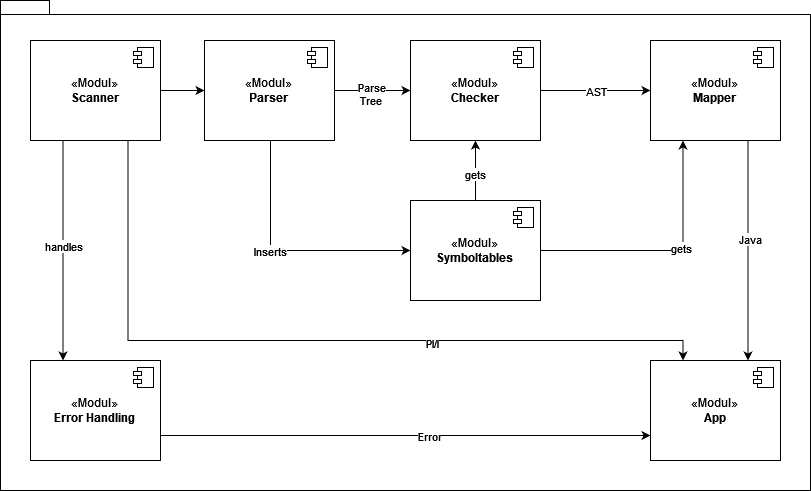
\includegraphics[scale=0.75]{AbstraktesUML_1.png}
	\label{fig:modules}
\end{figure}

% Wie sind die Module momentan gebaut?
% App Modul
Die Verarbeitung des PL/I-Quellcodes beginnt mit dem App-Modul. Das App Modul ist die Schnittstelle für alle weiteren Module. Ein Modul kann durch die Instanziierung der Hauptklasse des Moduls eingefügt werden. Entfernt wird das Modul durch das Löschen der Instanz. Das Modul beinhaltet auch die \verb+main+ Methode.

Der Scanner wird als erstes Instanziiert. Dieser liest aus der Config-Datei den Pfad der \verb+pli+ Datei, die übersetzt werden soll. Die Datei wird als \verb+InputStream+ an den Parser übergeben.

Der durch JavaCC erzeugte Parser wird ebenfalls in dem App-Modul instanziiert. Dieser behandelt den PL/I-Quellcode entsprechend der definierten Grammatik. Hier wird die Lexikalische und Syntaktische Analyse realisiert.

Während des parsings werden Variablen-, Prozeduren-, oder Packagebezeichner des PL/I-Quellcode, in die Symboltabelle eingefügt. Diese wird in dem Parser Modul zum ersten mal instanziiert. 

Das Ergebnis des Parsers ist ein Parsebaum.
Ist der Parsebaum erstmal entsprechend erzeugt, wird dieser weiterhin durch das Checker Modul verarbeitet. In diesem Modul wird die semantische Analyse des Quellcodes durchgeführt. Dabei wird auch die Symboltabelle verwendet um die Referenzen der Bezeichner im Quellcode auf korrketheit zu überprüfen. Teilweise ist es notwendig den Parse-Baum umzustellen. Ist der Parse-baum korrekt, oder korrekt verarbeitet worden, kann dieser als Abstrakter-Syntax-Baum (AST) im Mapper-Modul verwendet werden.

% @todo: Hier erwähnen wie Configdatei bzw. Scanner den Ausgabe Ordner beeinflussen wenn das implementiert wurde.
Das Mapper-Modul repräsentiert die Synthese des PL/I-Quellcodes. Der AST wird hier Stück für Stück abgearbeitet und mit entsprechenden Java-Ausdrücken übersetzt. Schlussendlich wird in dem \verb+target+ Ordner das übersetzte Programm abgelegt.
 
Ist das Programm fertig übersetzt kann der Java-Zielcode und die nötigen Klassen aus dem target Ordner exportiert werden und kompiliert, bzw. gewartet werden.

% Wie sind Module zueinander abhängig?
Jedes Modul führt zu der eigentlichen Ausgabe des Transpilers. Fehlt ein Modul kommt es automatisch zu Fehlern. 
Somit wird für eine korrekte Ausgabe jedes Modul benötigt.
Jedoch werde

% @todo: Hier UML 


% Wie wird es erweitert?


%Bausteine
%- Software Architektur
	%- Planen mithilfe eines UML
	%- UX Design 
    %    - zweite Diagramm, des Benutzerfluss
    %    - wie Benutzung abläuft
	%	- Website?
	%	- Docker Container?
%- Fehlertracking
%- Struktuierung des Programms, sodass ein Benutzer es selbständig erweitern kann

\subsection{Aspektorientierte Programmierung}
%- Wie funktioniert Aspektorientiert Programmierung?
%	- Wie Löse ich mit Aspektorientierter Programmierung konkrete Probleme?
%- JavaBeans
%- Spring
%	- Wie setzt Spring Aspektorientierte Programmierkonzepte ein?
 
\subsection{Module des Transpilers}
\subsubsection{Compiler-Compiler und Scanner}
Wie Kapitel 1.? eingeführt wird der Parser vollständig durch JavaCC generiert.
Um dennoch an die Konfigurationsdatei des Projektes zu gelangen wird ein Modul benötigt welches,
die Konfigurationsdatei und den Pfad zu der PL/I-Datei erfasst. Das Modul Scanner erfüllt diese Aufgabe.
  
\paragraph{Scanner}

% @todo: Nochmal überarbeiten, wenn neues dazukommt.
In dem App-Modul wird zuerst der Scanner instanziiert. 
Das Scanner Modul besteht aus den Klassen \verb+InputReader+ und \verb+Lexer+. 
Die \verb+InputReader+ Klasse liest die Konfigurationsdatei ein und speichert den Pfad, der mit der Variable \verb+PATH+
hinterlegt ist. Ein Ausschnitt einer möglichen Konfigurationsdatei ist in Listing ?.? hinterlegt.

\begin{verbatim}
	PATH=./src/main/java/res/pli/NPP1NFG.pli;
\end{verbatim}

Die Methode \verb+getInputFilePath+ liest die Konfigurationsdatei mithilfe eines Parameters der einem gültigen Pfad, zu einer Konfigurationsdatei,
entsprechen muss. Die Konfigurationsdatei ist in dem Ordner \verb+/res/config/+ hinterlegt. 
Die Methode ergibt den Pfad der \verb+.pli+ Datei als String. Dieser String wird beim Aufruf der \verb+getInputFile+ Methode benötigt. Diese ist ebenfalls Bestandteil der \verb+InputReader+ Klasse. Diese Methode ergibt wiederum einen InputStream der für das Parser-Modul für die weitere Bearbeitung des PL/I-Quellcode benötigt wird. Die Klasse \verb+InputReader+ ist für die Verarbeitung der Konfigurationsdatei und der Eingabe des PL/I-Quellcodes verantwortlich.

\paragraph{Lexer}
% @todo: Name von Lexer ventuell ändern, checken wegen install_id ob das so stimmt.
Die Klasse Lexer des Moduls Scanner enthält den ehemals selbst geschriebene Lexer für die lexikalische Analyse. Dadurch das dieser Prozess nun vollständig von dem JavaCC-Parser übernommen wird, wurde die Methode \verb+getToken+ überflüssig. Diese ist als veraltet mit der Kennung 'Deprecated' beschrieben, sie kann somit im Projekt noch verwendet werden, jedoch mit einem gewissen Risiko das die Ergebnisse der Methode nicht korrekt sind. Zu einem späteren Zeitpunkt ist denkbar den selbstgeschriebenen Lexer zu optimieren und erneut einzubinden. Weitere Methoden in dieser Klasse werden ebenfalls nicht länger von Klassen aus anderen Modulen verwendet. 

\paragraph{Parser}
% Was macht/Wie funktioniert der Parser für den Transpiler?
Der selbe Prozess der ursprünglich von dem Lexer gehandhabt wurde, wird nun von dem JavaCC Parser wahrgenommen. 
Dieser fügt nun die Bezeichner während der lexiklaischen- und syntaktischen Analyse in die Symboltabelle ein.
Aktuell wird deshalb mit der Methode \verb+installIds+ ein Bezeichner einer Variable, Methode oder Package in die Symboltabelle eingefügt.

Der Parser wird über die Klasse \verb+Pl1Parser+ instanziert. In dieser Klasse sind auch jegliche manuell geschriebenen Methoden aus der Grammatikdatei definiert. Dazu gehören etwas die eingangs beschriebene Methode \verb+installId+, sowie Getter und Setter-Methoden für benötigte Variablen, die während der Parser generierung initalisiert werden sollen. Wie etwa die Varialbe \verb+scope+ die beschreibt ob eine Variable Global oder Lokal instalisiert wurde.
Die Klasse \verb+Pl1Parser+ besteht vollständig aus Methoden, die in der Grammatikdatei verwendet wurden um eine Regel für einen Ausdruck festzulegen.
Listing ?.? zeigt so eine Methode für eine Prozedur in PL/I.

\begin{verbatim}
void procedure() #PROC :
{}
{
    proc_head()
    proc_body()
  	< END >< PL1_WORD >
}
\end{verbatim}

Die gleiche Methode ist in der Klasse \verb+Pl1Parser+ zu finden. Hier in Listing ?.? zu sehen.

\begin{verbatim}

final public void procedure() throws ParseException {/*@bgen(jjtree) PROC */
  
  SimpleNode jjtn000 = new SimpleNode(JJTPROC);
  boolean jjtc000 = true;
  jjtree.openNodeScope(jjtn000);
    
  try {
      
      proc_head();
      proc_body();
      jj_consume_token(END);
      jj_consume_token(PL1_WORD);
    
	} catch (Throwable jjte000) {
	 if (jjtc000) {
        	jjtree.clearNodeScope(jjtn000);
        	jjtc000 = false;
      		} else {
		...
      		} finally {
      			if (jjtc000) {
        			jjtree.closeNodeScope(jjtn000, true);
      			}
    		}
	}
}
\end{verbatim}

Zu erkennen ist das auch hier die beiden Methoden wie in Listing ?.? aufgerufen werden. (Zeile ? und ?)
Daraufhin folgt in Listing ?.? die Verwendung des \verb+END+ und des \verb+PL1_WORD+ Tokens.
In Listing ?.? werden diese als Parameter an die \verb+jj_consume_token+ Methode übergeben.
Die Tokens werden in der Klasse \verb+Pl1ParserConstants+ als Konstanten definiert.
Die Methode \verb+jj_consume_token+ wird verwendet um die Tokens mithilfe der Klasse \verb+Token+ und \verb+TokenMgrError+ zu verarbeiten.
Ist der Ausdurck nicht zulässig wird eine ParseException geworfen, die in der Klasse \verb+ParseException+ definiert ist.
Gelesen wird der Token durch die Klasse \verb+SimpleCharStream+. Um den Ausdruck in einem Parse-Baum zu repräsentieren wird ein Objekt der Klasse \verb+SimpleNode+ erzeugt. Durch die Methoden \verb+clearNodeScope+ und \verb+closeNodeScope+ der Klasse \verb+JJTPl1ParserState+ wird der verarbeitete Ausdruck mit der repräsentation \verb+PROC+ in den Prasebaum eingefügt. In den anderen \verb+if else+ Verwźweigungen von Zeile ? bis ?, werden Exception abgefragt und ensprechende Fehlermeldungen geworfen.
So verarbeitet der Praser des Transpilers Stück für Stück die PL/I Ausdrück. Hat der Parser einen Bezeichner gefunden, wird die Methode \verb+installIds+ aufgerufen. Diese wird lediglich durch die JavaCC Methode \verb+id+ aufgerufen, welche in listing ?.? abgebildet ist.

\begin{verbatim}
  final public void id() throws ParseException {/*@bgen(jjtree) Id */
 ...
    try {
      t = jj_consume_token(PL1_WORD);
...
String[] tmp = {t.image, this.getHierachie() + "", this.scope + "","id"};
        this.installIds(tmp);
...
}\end{verbatim}

Ein Bezeichner kann nur unter bestimmten Bedingungen in die Symboltabelle eingefügt werden. Ein Bezeichner wird nicht eingefügt, 
wenn dieser schon vorhanden ist und eine gleiche Sichtbarkeit hat. Ist das nicht der Fall wird die Variable eingefügt.

\subsubsection{Symboltable}
Die Symboltabelle wird verwendet um Bezeichner korrekt aus dem PL/I-Quellcode zu extrahieren und in den Java-Zielcode in installieren.
Das Modul \verb+Symboltable+ enthält die Klassen \verb+SymbolTable+, \verb+Pl1Symbols+ und \verb+PictureMapper+.
Zusätzlich enthält das Modul die Enums \verb+Pl1Symbols+ und \verb+Template+.

% Wie funktioniert SymbolTable und Pl1Smybols?
Die Klasse \verb+SymbolTable+ wird beim instanziieren des Objekts mit den Werten aus dem Enum \verb+Pl1Symbols+ inistallisiert. 
Bei der Datenstruktur der Symboltabelle handelt es sich um eine Hashtabelle. Ein Integer wird als Id verwendet und ein String Array um die Daten über die Variable bzw. das Wort zu Speichern. 
Wenn ein Bezeichner in die Symboltabelle eingefügt wird müssen, ein String für den Bezeichner, ein String für den Typ, ein Integer für die Sichtbarkeit und ein Integer für die Hierachiestufe der Variable hinterlegt sein. Nur so können andere Module wie der Parser, die Werte korrekt verarbeiten.
Der Parser verwendet die Symboltabelle etwa dazu, diese zu durchzuchen und um festzustellen ob der Wert bereits eingefügt wurde.
Dies kann der Fall sein, wenn der Bezeichner ein PL/I-Token ist oder während des übersetzens ein gleicher Wert eingefügt wurde.
Dann sollte die Methode, in der die \verb+insert+ Methode der \verb+Symboltable+ Klasse eine Fehlermeldung werfen.
Die Methode \verb+getSymbolScope+ wird dazu verwendet den Sichtbarkeitswert eines Bezeichners auszugeben. Das ermöglicht eine dedizierte,
abwägung wie dieser Wert verwendet werden soll. Diese Methode wird in dem Checker Modul in Kapitel ?.? erneut betrachtet.
Restliche Methoden sind hauptsächlich dazu da, Symbole gezielt abzufragen oder in der Konsole auszugeben.

% Wie funktioniert Template?
Der weitere Enum \verb+Template+ dient, in einem der folgenden Prozessschritte den Abstrakten-Syntax-Baum in Java-Code umzuwandeln.
In diesem Enum sind Java-Quellcode Ausschnitte hinterlegt die PL/I-Quellcode repräsentieren können. Sie werden in dem Mapper Modul verwendet
um nach und nach den Java-Zielcode zu erzeugen.

% Wie funktioniert der PicturemMapper
Die Klasse \verb+PictureMapper+ enthält ebenfalls eine Hashmap, hier befinden sich Zeichen die Ausdrücke des Picture Typs aus PL/I und deren übersetzugn als Regulären Ausdruck. 
Mit der \verb+getRegex+ Methode der \verb+PictureMapper+ Klasse wird der Picture Ausdruck übersetzt und als String zurückgegeben.
Der Ausdruck \verb+(4)A+ wird etwa zu \verb+(A-Za-z ){4}+. Dadurch kann die Beschränkung der Länge des Strings, des Picture-Typs im Java-Zielcode beibehalten werden. 
Verwendet wird diese Klasse hauptsächlich von dem Mapper-Module, wenn der Abstrakte Syntaxbaum in Java übersetzt wird.

Um den Abstrakten Syntax Baum zu erzeugen muss der Parsebaum Stück für Stück überprüft werden. Dieser Prozess wird als semantische Analyse bezeichnet und erfolgt im Checker Modul. 
\subsubsection{Checker}
\subsubsection{Mapper}
\subsubsection{Error-Handling}

\subsection{Testing und Integration}
%1. Transpiler wird getestet
%1.1 Testen der Methoden von Lexer, Parser usw. (Bsp.: Kann dieses Zeichen verarbeitet werden?)
%1.2 Baum testen auf Korrektheit

%2. Transpilieren wird getestet
%2.1 Output des transpilierten Pl/1 Codes im Verhältnis zum Pl/1 Code testen.

%3. Der Transpilierte Code wird getestet
%- Wie wird PL/1 Code Native getestet
%- Funktioniert der Java Code richtig

%4. Performance Test (erst am ende)

\subsection{Fehlerbehandlung}
Um dem Benutzer die Bediengung während der Laufzeit zu erleichtern, wurden Selbstgewählte Fehlermeldungen implementiert. Diese Fehlermeldungen sollen den Benutzer der Software in eine Feedback schleife bringe welche klare Anweisung zur Bediengung gibt. In der usprünglichen Version des Transpilers wurde dem Benutzer lediglich die von Java geworfenen Fehler in der Konsole ausgegeben. Die Fehlermeldung"IndexOutOfBounds", ließ dabei nicht darauf schließe das der Transpiler die PL/I Datei zum lesen nicht findet. Eine solche Fehlermeldung führt erneut dazu, dass der Benutzer sich selbst um die Lösung des Problems kümmern musste und somit einer weiteren Hürde begenete.
Eben für dan Fall das die Datei nicht gelesen werden kann, wurde eine Exception geschrieben. Die Exception "PliFileNotFound", beschreibt dem Benutzer die Ursache des Problems und nennt auch ein etwaaigen Lösungsvorschlag. Es exstieren in der neusten Version einige Exceptions die in der folgenden Tabelle näher Beschrieben werden.

...Tabelle mit Exceptions...

Fehlerbehandlung spielt besonder im Zusammenhang mit der Lexikalischen Analyse eine Rolle. Um zu gewährleisten das die Transformation korrekt albläuft braucht es der formalen PL/I Grammatik enstrpechend richtigen PL/I Code als Eingabe. Eine nicht behandlung hätte zur Folge das das Programm entweder eine Fehlerhafte Ausgabe produziert, oder Fehlschlägt. Dies soll vermieden werden.

\section{Technische Spezifikation}
	\subsection{Ausführung des Transpilers}
		\subsubsection{Transformationsmöglichkeiten}
		%Toleranzspielräume:...Einfach, Genau, Präzisse
		\subsubsection{Umwandlung von Datentypen}
		\subsubsection{Umwandlung von Prozeduren}
	\subsection{Optimierung}
	% Online-Smoketest von PL/I Code -> %todo: Verschieben nach Erweiterbarkeit (Schlusskapitel), weil momentan noch nicht vollständige Grammatik realisiert.
	Ein weiterer denkbarer Einsatzbereich ist es, den PL/I-Code auf seine Richtigkeit zu testen. Wird mithilfe des Programms erfolgreich das PL/I-Programm in Java übersetzt, so sollte auch ein herkömmlicher PL/I-Compiler auf einem Mainframe den Code ausführen können. Somit eignet sich das Programm auch für Smoke-tests von Anwendungen.
		\subsubsection{Performance und Benchmarks}
		\subsubsection{Testing}
